\documentclass[conference]{IEEEtran}
\usepackage{cite}
\usepackage{amsmath,amssymb,amsfonts}
\usepackage{algorithmic}
\usepackage{graphicx}
\usepackage{textcomp}
\usepackage{xcolor}
\usepackage{url}
\usepackage{hyperref}
\usepackage{booktabs} % For better table formatting
\usepackage{svg}
\def\BibTeX{{\rm B\kern-.05em{\sc i\kern-.025em b}\kern-.08em
    T\kern-.1667em\lower.7ex\hbox{E}\kern-.125emX}}



\hyphenpenalty=5000
\exhyphenpenalty=5000
\sloppy
\begin{document}
\IEEEpubid{\makebox[\columnwidth]{XXX-X-XXXX-XXXX-X/XX/\$XX.00~\copyright20XX IEEE \hfill} \hspace{\columnsep}\makebox[\columnwidth]{ }}

\title{An AI-Driven Personalized Sinhala Teaching Assistant for Secondary Education Using Curriculum Aligned Large Language Models}

\author{}

\maketitle

\begin{abstract}
Sri Lanka faces a shortage of qualified teachers, with rural regions being disproportionately affected, resulting in unequal learning opportunities for students preparing for the General Certificate of Education Ordinary Level (GCE O/L) and Advanced Level (GCE A/L) examinations. Existing digital learning platforms primarily provide static, prerecorded content and lack adaptive personalization, while general-purpose Large Language Models (LLMs) are not aligned with the national curriculum. This paper presents an Artificial Intelligence (AI)-driven Sinhala teaching assistant that integrates four components: (i) a curriculum-aligned Sinhala LLM (SinLlama-8B) for educational content generation, (ii) a Hybrid Bayesian Knowledge Tracing (Hybrid-BKT) framework combining Personalized Clustered Bayesian Knowledge Tracing with Long Short-Term Memory (LSTM)-based temporal modeling for learner mastery estimation, (iii) a Retrieval-Augmented Generation (RAG) pipeline supported by a ChromaDB indexed national syllabus content embedded via multilingual-e5-base, and (iv) a LangGraph-orchestrated multi-agent architecture for coordinated instructional support. SinLlama-8B outperforms Qwen-14B, Llama-3.1-8B, DeepSeek-14B, and Mistral-7B in curriculum alignment and semantic fidelity. The Hybrid-BKT framework continuously estimates learner knowledge states, enabling adaptive content delivery tailored to individual proficiency levels. The production system employs a dual-LLM architecture: the fine-tuned SinLlama model handles curriculum grounded content generation through RAG, while general-purpose LLM (Llama-3.3-70B via Groq) powers rapid agent orchestration. Experimental results demonstrate the feasibility and effectiveness of integrating curriculum-aligned language models, knowledge tracing, and retrieval-augmented generation for personalized secondary education in Sri Lanka. Additionally, an interactive AI Avatar powered by Gemini Text To Speech (TTS) delivers spoken Sinhala lesson explanations.
\end{abstract}

\renewcommand\IEEEkeywordsname{Keywords}
\begin{IEEEkeywords}
Bayesian knowledge tracing, Intelligent tutoring systems, Personalized Learning Systems, Retrieval-augmented generation (RAG), Sinhala natural language processing (NLP)
\end{IEEEkeywords}
\vspace{-1em}
\section{INTRODUCTION}
Education is widely recognized as a cornerstone of human development, yet students preparing for the General Certificate of Education Ordinary Level (G.C.E. O/L) and Advanced Level (G.C.E. A/L) examinations in Sri Lanka face severe systemic challenges. The country faces a shortage of more than 30,000 qualified teachers, causing student-to-teacher ratios to exceed 50:1, with the problem disproportionately affecting rural provinces \cite{b1}. These conditions perpetuate a stark divide in educational quality between urban and rural learners. Statistically, only 63.3\% of O/L candidates qualify for A/L studies, blocking over 130,000 students annually from tertiary education pathways, while a mere 15\% of A/L candidates secure university admission \cite{b2}. 

Several digital platforms have attempted to bridge this divide. The government-sponsored e-Thaksalawa portal \cite{b3} and private initiatives such as Dammika Perera (DP) Education offer pre-recorded video lectures, downloadable notes, and fixed question banks but lack the adaptive, interactive dimension necessary for effective personalized tutoring. General purpose Large Language Models (LLMs), while increasingly capable in Sinhala, are not aligned with the Sri Lankan national curriculum and tend to generate generic responses inappropriate for exam preparation \cite{b4}.

These observations point to a research gap that, to the best of our knowledge, has not been addressed in the literature: The absence of an Artificial Intelligence (AI) based educational system that (a) operates natively in the Sinhala medium, (b) strictly adheres to national syllabus content, (c) dynamically adapts to each student's evolving knowledge state, and (d) provides verifiable, curriculum-grounded responses rather than unchecked generative output, are the observations that point to the research gap.

The work is guided by four research questions investigating: (i) the effectiveness of different LLM architectures in achieving high semantic fidelity for curriculum-aligned Sinhala content generation after fine-tuning on national syllabus data, (ii) whether a hybrid ensemble combining Personalized Clustered BKT and LSTM-based temporal modeling improves student mastery estimation compared to conventional BKT approaches, (iii) the extent to which a RAG pipeline grounded in vectorized syllabus content can constrain model outputs within curriculum boundaries, and (iv) the ability of a multi-agent architecture to effectively orchestrate personalized and adaptive learning workflows for secondary-level education. Finally, a deployed web and mobile prototype is presented to demonstrate practical applicability.

The remainder of this paper is organized as follows. Section II reviews related work across intelligent tutoring systems, adaptive learning, LLMs in education, RAG, and multi-agent architectures. Section III details the system methodology, Section IV reports experimental results. Section V discusses findings and limitations, and Section VI concludes with directions for future work.

\section{RELATED WORK}
This section reviews five areas of related research: intelligent tutoring systems, adaptive learning and student modelling, generative AI and LLMs in education, retrieval-augmented generation for education, and multi-agent tutoring architectures.

\subsection{Intelligent Tutoring Systems}
Intelligent Tutoring Systems (ITS) employ machine learning, educational data mining, and adaptive assessment to personalize instruction \cite{b6}. Xu et al. \cite{b7} demonstrated that AI-driven adaptive learning frameworks significantly improve engagement, assessment scores, and knowledge retention compared to non-adaptive systems. However, most ITS implementations target English-language learners via text-only interaction, leaving low-resource language contexts underserved \cite{b8}.

\subsection{Adaptive Learning and Student Modeling}
BKT introduced by Corbett and Anderson \cite{b9}, remains the most widely adopted student modelling framework. BKT estimates the probability of knowledge mastery through a Hidden Markov Model parameterized by four parameters: Prior knowledge $P(L_0)$, learning rate $P(T)$, guess rate $P(G)$, and slip rate $P(S)$. However, standard BKT assumes uniform learner priors and fixed parameters, limiting its capacity for personalized student modelling. 

Several extensions address these limitations. Nedungadi and Remya \cite{b10} proposed Personalized Clustered BKT (PC-BKT), combining K-Means based student clustering with empirically estimated BKT parameters to improve cold-start predictions. Minn \cite{b11} combined BKT with LSTM networks (BKT-LSTM), capturing temporal learning dynamics beyond the Markov assumption.

\subsection{Generative AI and LLMs in Education}
Recent systematic reviews confirm that LLMs such as GPT, BERT, and T5 offer significant potential for personalized learning, adaptive feedback, and intelligent tutoring \cite{b12}. Kasneci et al. \cite{b13} highlighted both the promise and risks of ChatGPT in education, noting its tendency to hallucinate and its lack of curriculum alignment.

For low resource languages such as Sinhala, the availability of pre trained language models has improved with the development of SinLlama \cite{b5}, a 7-billion-parameter model specifically pre trained on Sinhala text corpora. However, no prior work has fine-tuned SinLlama or any Sinhala LLM on national curriculum content for structured examination preparation. These limitations motivate the need for curriculum-grounded, language-specific fine-tuning as pursued in this work.

\subsection{Retrieval-Augmented Generation for Education}
RAG combines information retrieval with generative models to reduce hallucinations and improve factual grounding. The foundational RAG framework was introduced by Lewis et al. \cite{b14} demonstrating that conditioning generation on retrieved documents substantially improves knowledge-intensive NLP tasks. Li et al. \cite{b15} systematically reviewed RAG techniques for education, noting their suitability for curriculum based adaptive learning. However, existing RAG based educational systems focus almost entirely on English and higher education contexts. Applying RAG to Sinhala medium secondary school education where textbooks must be digitized, segmented, and embedded in a low resource language pipeline remains unexplored.

\subsection{Multi-Agent Systems for Tutoring}
Multi-agent architectures distribute teaching tasks among specialized agents, improving system scalability and pedagogical flexibility. David and Ghosh \cite{b16} introduced IntelliCode, a StateGraph based orchestration architecture with centralized learner memory that enables long-term student tracking across multiple tutoring sessions. The LangGraph framework \cite{b17} extends LangChain with stateful, graph-based orchestration of multi agent workflows, built-in checkpointing, and conditional routing making it well-suited for adaptive educational applications that require persistent student state management.

\subsection{Summary of Research Gaps}
A review of existing systems reveals several significant gaps in Sinhala-medium intelligent tutoring systems. To the best of our knowledge, no existing solution system simultaneously integrates Sinhala medium instruction, national curriculum alignment, adaptive student modelling, RAG-based content grounding, and multi agent orchestration within a unified educational framework.

\section{METHODOLOGY}
\begin{figure*}[t]
\centerline{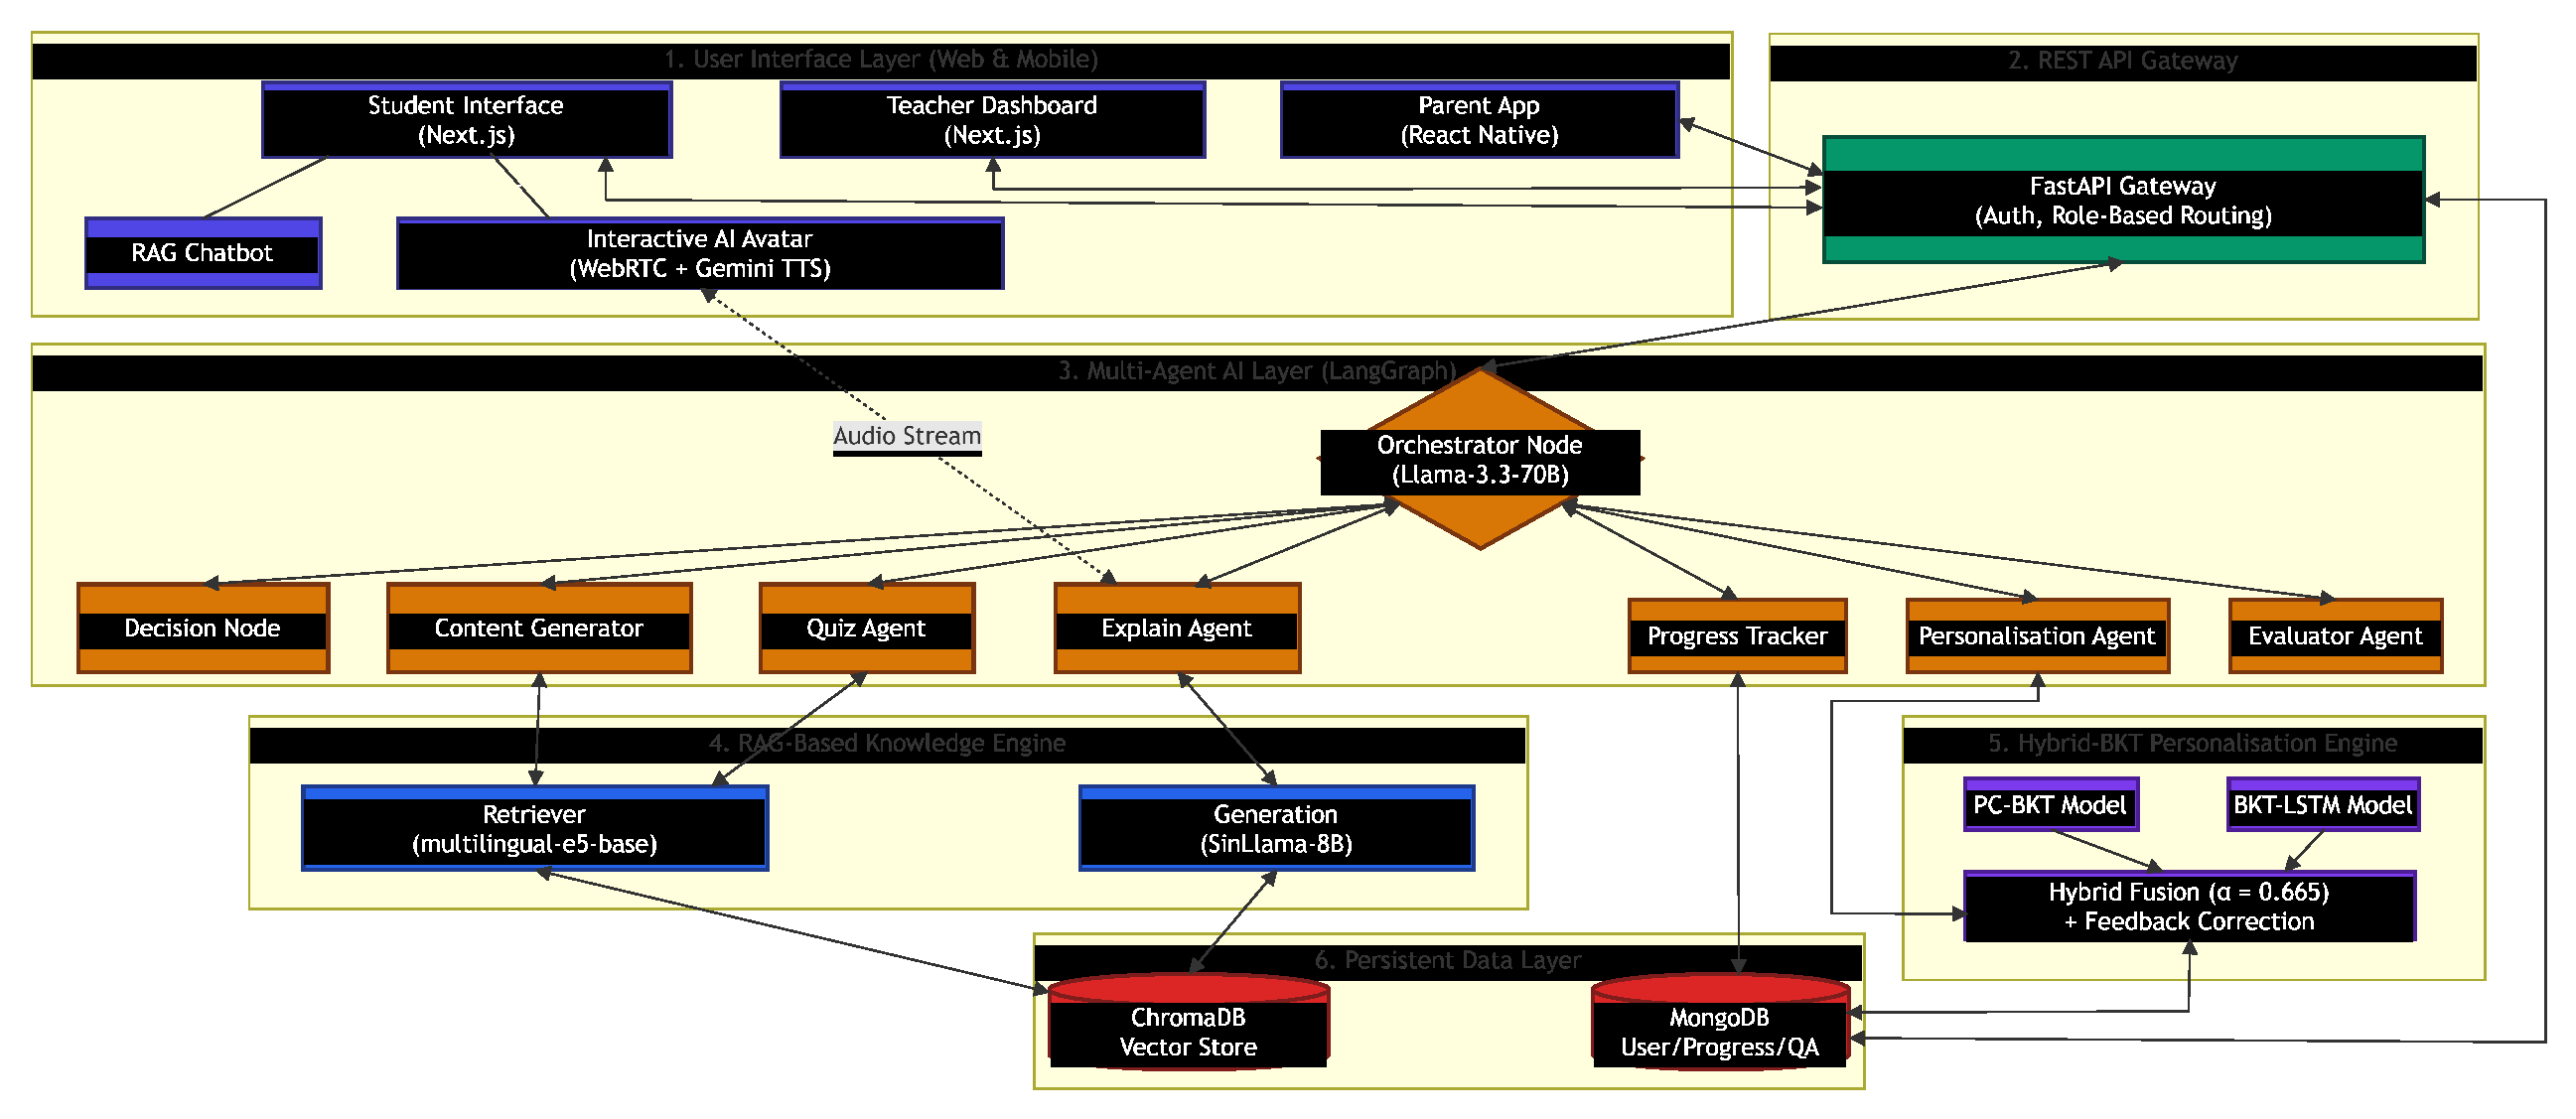
\includegraphics[width=\textwidth,height=7cm]{architecture.pdf}}
\caption{System Architecture Diagram}
\label{fig1}
\end{figure*}
\subsection{System Architecture Overview}
The system is a fully implemented and deployed as a web application (Next.js) and mobile application (React Native / Expo), featuring an interactive AI Avatar teacher powered by Gemini Text To Speech (TTS) and WebRTC based real time video streaming, a RAG powered conversational chatbot, a teacher analytics dashboard, and a parent monitoring module. 

The proposed system follows a modular architecture comprising six integrated layers. The functionality of each layer is described below:

1) User Interface Module - Three role-specific interfaces served across web and mobile platforms.

\textit{Student Interface}: provides lesson browsing with hierarchical navigation, pre-quiz and post-quiz sequences with real-time adaptive feedback, conversational chatbot for Sinhala Q\&A and an interactive AI Avatar teacher that delivers spoken lesson explanations.

\textit{Teacher/Admin Dashboard}: visualizes per-student quiz performance trends, topic-wise mastery levels, lesson completion percentages, and engagement session histories.

\textit{Parent Mobile Interface}: provides child progress summaries.

2) REST API Gateway - Client–server communication flows through well-defined endpoints implemented with Python FastAPI.

3) Multi-Agent AI Layer - Seven task specific agents orchestrated via a LangGraph StateGraph supervisor for adaptive workflow management.

4) RAG-based Knowledge Engine - Retrieval pipeline that grounds all generated content in vectorized Sinhala textbooks.

5) Hybrid BKT Student Modelling Engine - A personalization engine combining PC-BKT with LSTM-based temporal prediction for mastery estimation and adaptive content delivery.

6) Persistent Data Layer - MongoDB for store user profiles, student progress, interactions sessions and logs.

Each layer communicates through well-defined REST API endpoints implemented with FastAPI, ensuring horizontal scalability and component modularity. Fig. 1 illustrates the data flow between layers.

\vspace{-0.5em}
\subsection{LLM Fine-Tuning for Sinhala Education}
\vspace{-0.5em}
To identify the most suitable model for Sinhala content generation, five Sinhala-supporting LLMs were evaluated. SinLlama-8B, Qwen-14B, Llama-3.1-8B, DeepSeek-14B, and Mistral-7B. All five LLMs were fine-tuned on the Buddhism Questions and Answers dataset using Low-Rank Adaptation (LoRA) \cite{b18} to enable training on consumer-grade hardware.

All models were fine-tuned on this dataset and evaluated using ROUGE scores, BERTScore, token generation speed, and an LLM-as-a-Judge protocol, where a larger-parameter LLM acted as the evaluator and assigned scores out of 20 based on Accuracy, Completeness, Clarity, and Depth. The model demonstrating the best overall performance in the evaluation phase was subsequently selected for integration into the proposed system.

\subsection{Retrieval-Augmented Generation Pipeline}
The RAG pipeline ensures all generated content remains grounded in verified curriculum resources, thereby mitigating the hallucination risks commonly associated with standalone generative language models.

(i) The knowledge base was constructed from Sinhala-medium educational resources, including official textbooks, teacher guidance manuals, and past examination papers. Source documents were digitized using Optical Character Recognition (OCR) and subsequently verified to ensure textual accuracy. To preserve semantic continuity while enabling efficient retrieval, documents were segmented into overlapping chunks of 512 tokens with an overlap of 64 tokens.

(ii) Each document chunk was encoded using the intfloat/multilingual-e5-base sentence transformer model, producing 768-dimensional dense vector representations. The resulting embeddings were indexed using ChromaDB.

(iii) During inference, student queries and assessment answers were embedded through the same model as that of the documents and matched to the indexed document repository. The top five document chunks similar to the vector were retrieved and used in the generation prompt. Mastery awareness-based prompting was adopted in the process, combining the learner's level of mastery. This approach enables the framework to facilitate generation of pedagogically appropriate responses by adding context to generation with the curriculum-relevant information.

The retriever supports two complementary retrieval modes: (a) a document order mode for lesson content generation that fetches all chunks matching the source file and sorts by paragraph index to preserve narrative coherence, and (b) a vector similarity ranking mode for quiz generation. 

The backend FastAPI server mounts a static images directory, enabling the Next.js frontend to dynamically render these illustrations inline with the retrieved text, maintaining a multimodal learning experience.

\subsection{Hybrid-BKT Personalization Engine}
The personalization engine uses a weighted ensemble of two complementary models: Personalized Clustered Bayesian Knowledge Tracing (PC-BKT) and a BKT-LSTM temporal predictor.

\textit{(a) \underline{PC-BKT}:} Standard BKT is a Hidden Markov Model tracking a student's latent knowledge state using four parameters: initial mastery $P(L_0)$, learning transition $P(T)$, guess rate $P(G)$, and slip rate $P(S)$.

When a student interacts with the system at timestep $t$, the correctness $C_t \in \{0, 1\}$ the mastery probability $P(L_t)$ will be updated.

\textit{Correct response Update:}
{\small
\begin{equation}
P( L_t \mid C_t = 1 ) = \frac{P(L_{t-1})(1 - P(S))}{P(L_{t-1})(1 - P(S)) + (1 - P(L_{t-1}))P(G)}
\end{equation}
}

\textit{Incorrect response Update:}
{\small
\begin{equation}
P( L_t \mid C_t = 0 ) = \frac{P(L_{t-1})P(S)}{P(L_{t-1})P(S) + (1 - P(L_{t-1}))(1 - P(G))}
\end{equation}
}

\textit{Learning Transition Update:}
{\small
\begin{equation}
P(L_{t+1}) = P(L_t \mid C_t) + (1 - P(L_t \mid C_t))P(T)
\end{equation}
}

PC-BKT \cite{b10} extends this by personalizing priors. First, initial mastery $P(L_0)$ is computed per knowledge component (KC) via Correct First Attempt rates. Second, students are clustered into three ability groups using K-Means++ on their performance capability matrix. Finally, $P(G)$, $P(S)$, and $P(T)$ are estimated empirically from interaction sequences rather than fixed presets.

\textit{(b) \underline{BKT-LSTM}:} The BKT-LSTM component \cite{b11} reformulates mastery prediction as a temporal sequence forecasting problem. At each interaction timestep $t$, a feature vector is constructed:
{\small
\begin{equation}
f(t) = [P(L)_{BKT}, d_{KC}, c_t, a_t]
\end{equation}
}
where $P(L)_{BKT}$ is the current standard BKT mastery probability, $d_{KC}$ is the normalized difficulty of the knowledge component, $c_t \in \{0, 1\}$ is the correctness indicator, and $a_t$ is the cumulative attempt count. 

It employs a two-layer stacked LSTM (128 hidden units) that takes the current BKT mastery probability, normalized KC difficulty, correctness indicator, and attempt count as inputs. This captures temporal learning patterns, forgetting effects, and cross-KC transfer not represented by standard BKT.

\textit{(c) \underline{Hybrid-BKT}:} The final student mastery estimate is calculated as a weighted ensemble:
{\small
\begin{equation}
P_{hybrid}(t) = \alpha P_{PC-BKT}(t) + (1 - \alpha)P_{LSTM}(t)
\end{equation}
}

Here, $\alpha \in [0, 1]$ represents the ensemble weight parameter that determines the relative contribution of the PC-BKT and BKT-LSTM models. The optimal value of $\alpha$ was determined to be 0.665 using a two-stage grid search designed to minimize the Root Mean Squared Error (RMSE) on a held-out validation fold. The weight $\alpha = 0.665$ was obtained by first running a coarse grid search over: $\alpha \in \{0.0, 0.05, \dots, 1.0\}$ which identified the local minimum in the range $[0.60, 0.70]$.

\textit{(d) \underline{LSTM-BKT Feedback Correction}:} To detect potential guessing behavior, the system monitors divergence between BKT and LSTM mastery estimates. When the BKT-derived mastery exceeds the LSTM prediction by more than a threshold $\delta = 0.20$, the system suspects that correct answers may have resulted from guessing rather than genuine understanding. In such cases, a negative feedback correction is applied:
{\small
\begin{equation}
P_{hybrid}(t) = P_{hybrid}(t) - 0.5(P_{PC-BKT}(t) - P_{LSTM}(t))
\end{equation}
}
This feedback mechanism addresses the known limitation of standard BKT, which cannot distinguish lucky guesses from true mastery when the guess rate $P(G)$ is high.

\subsection{Multi-Agent Orchestration}
The adaptive learning workflow is orchestrated by a LangGraph StateGraph supervisor that coordinates seven dedicated agents through conditional routing 
$\bullet$ \textit{\underline{The Orchestrator Node}:} the entry point for every learning request. Determines learner state and routes data based on quiz type, scoring completion, content availability, and mastery progression. After each agent completes, control returns to the Orchestrator for re-evaluation, creating an iterative refinement loop.

$\bullet$ \textit{\underline{The Evaluator Agent}:} grade students after submitting the answers. computes a normalized score (0–10 scale), and classify as Beginner (score $<$ 5), Intermediate (5 $\le$ score $<$ 8), or Advanced (score $\ge$ 8).

$\bullet$ \textit{\underline{Personalization Agent}:} the core of the adaptive engine. It executes the full Hybrid-BKT pipeline. computes hybrid mastery via weighted fusion, applies the LSTM - BKT feedback correction, and generates adaptive learning signals.

$\bullet$ \textit{\underline{Content Generator Agent}:} uses the RAG pipeline to produce mastery-aware personalized lessons.

$\bullet$ \textit{\underline{Quiz Agent}:} dynamically constructs five question multiple choice quizzes in Sinhala by sending RAG retrieved context to the fine-tuned model with curriculum aligned quiz generation prompts.

$\bullet$ \textit{\underline{Explain Agent}:} provides context-aware explanations by sending lesson content to SinLlama for simplified re-explanation. Also, strips image tags from content before processing and produces speakable text specifically designed for the Avatar TTS pipeline.

$\bullet$ \textit{\underline{Progress Tracker Agent}:} maintains persistent interaction logs, mastery histories, and engagement analytics in MongoDB.

All agents share a common state object managed by LangGraph, ensuring consistent learner context across transitions.

\subsection{Adaptive Assessment Cycle}
The proposed framework facilitates learning through four phases.

\textit{\underline{Phase 1 (Pre-Assessment)}:} Students complete a pre-quiz on a target knowledge component; questions are generated dynamically via an LLM-based pipeline aligned to Bloom's taxonomy (Remember, Understand, Apply), with one question per level drawn from curriculum metadata.

\textit{\underline{Phase 2 (Adaptive Content Generation)}:} The Evaluator Agent classifies mastery via $P_{hybrid}(t)$ and assigns one of the three tiers. Beginner ($P_{hybrid}(t) < 0.60$): foundational content with definitions, worked examples, and guided practice. Intermediate ($0.60 \le P_{hybrid}(t) < 0.85$): standard lesson with moderate scaffolding and application exercises. Advanced ($P_{hybrid}(t) \ge 0.85$): enrichment content with higher-order analysis and past-paper questions. The Evaluator Agent classifies mastery level and the Content Generator Agent produces a personalized lesson.

\textit{\underline{Phase 3 (Post-Assessment)}:} A post-quiz of equivalent difficulty measures updated mastery $P_{hybrid}(t+1)$. Students who meet the advancement threshold ($\ge 0.85$) progress to the next KC; those in the Intermediate range repeat the KC with alternative content; those below $0.60$ receive remedial material with simplified explanations.

\textit{\underline{Phase 4 (Continuous Adaptation)}:} Student interactions continuously update the capability matrix, while periodic retraining refines learner ability clusters to improve personalization over time.

\subsection{Interactive AI avatar Teacher}
To enhance learner engagement and simulate a classroom teaching experience, the system incorporates an interactive AI Avatar that delivers spoken Sinhala lesson explanations. The Avatar pipeline operates in three stages:

\textit{\underline{Stage 1}:} The Explain Agent processes RAG retrieved lesson content through SinLlama to produce a simplified, spoken form explanation with image tags stripped.

\textit{\underline{Stage 2}:} Text is synthesized into Sinhala speech using Google Gemini TTS (gemini-2.5-flash-preview-tts, 24 kHz) and delivered to a lip-synced 3D avatar via WebRTC streaming, enabling real-time spoken lesson delivery with selectable avatar identities.

\textit{\underline{Stage 3}:} Sentence tracking mechanism synchronizes text highlighting on the frontend with the avatar's estimated speech progress.

\section{RESULTS}
\subsection{LLM Evaluation}
Five Sinhala-supporting LLMs were fine-tuned on the Buddhism curriculum question and answering (QA) dataset comprising 3,547 QA pairs. The dataset was synthetically generated using AI based on the national subject content and curriculum materials provided for the Buddhism syllabus. The models were evaluated using ROUGE scores, BERTScore, token generation throughput (measured as the number of tokens generated per second), and an LLM-as-a-Judge evaluation protocol, where a separate LLM was employed to assess the quality, correctness, relevance, and pedagogical appropriateness of generated responses according to predefined evaluation criteria.

The evaluation was conducted on a held-out test set of 532 QA pairs (15\% of the dataset), stratified by topic to ensure coverage across all KCs. The results have been obtained by calculating the average performance across three runs of fine tuning with random seeds.

Table I presents ROUGE scores for all the tested five models. SinLlama-8B demonstrates the best overall performance across all ROUGE metrics, achieving ROUGE-1 of 0.7714, ROUGE-2 of 0.6418, and ROUGE-L of 0.6111. It significantly outperforms the next-best baseline, Mistral, which records a ROUGE-1 score of 0.4925. Table II presents the BERTScore results, where SinLlama-8B achieves the highest score of 0.9424, consistently outperforming Llama-3.1, DeepSeek-14B, Mistral-7B, and Qwen-14B, with scores of 0.8799, 0.8659, 0.8555, and 0.8022, respectively. In the LLM-as-a-Judge evaluation (Table II), SinLlama-8B achieved the highest overall score of 15.88/20, followed by Mistral-7B with 14.97/20. DeepSeek demonstrated the fastest token generation (444.9 tokens/sec) but lower semantic accuracy, making it suitable only for latency-critical deployments where accuracy is secondary.
\vspace{-1.0em}
\begin{table}[htbp]
\caption{ROUGE Scores of Evaluated LLMs}
\vspace{-1.5em}
\label{tab1}
\begin{center}
\begin{tabular}{lccc}
\toprule
\textbf{Model} & \textbf{ROUGE-1} & \textbf{ROUGE-2} & \textbf{ROUGE-L} \\
\midrule
SinLlama-8B & \textbf{0.7714}* & \textbf{0.6418}* & \textbf{0.6111}* \\
Qwen-14B & 0.3310 & 0.1678 & 0.1059 \\
Llama-3.1-8B & 0.3983 & 0.1949 & 0.1418 \\
DeepSeek-14B & 0.4485 & 0.2304 & 0.1845 \\
Mistral-7B & 0.4925 & 0.2280 & 0.1594 \\
\bottomrule
\multicolumn{4}{l}{$^{\mathrm{*}}$ Statistically significant vs. all other models ($p < 0.001$).}
\end{tabular}
\end{center}
\end{table}
\vspace{-1.5em}
\begin{table}[htbp]
\caption{BERTScore and LLM-as-a-Judge Evaluation}
\vspace{-1.5em}
\label{tab2}
\begin{center}
\resizebox{\columnwidth}{!}{
\begin{tabular}{lccccc}
\toprule
\textbf{Model} & \textbf{BERTScore} & \textbf{Accuracy} & \textbf{Clarity} & \textbf{Depth} & \textbf{Total/20} \\
\midrule
SinLlama-8B & \textbf{0.9424} & \textbf{4.78} & \textbf{4.50} & 2.38 & \textbf{15.88} \\
Mistral-7B & 0.8555 & 4.50 & 4.34 & \textbf{2.53} & 14.97 \\
Llama-3.1-8B & 0.8799 & 4.28 & 4.34 & 2.25 & 13.59 \\
DeepSeek-14B & 0.8659 & 4.22 & 4.36 & 2.09 & 13.58 \\
Qwen-14B & 0.8022 & 2.97 & 4.34 & 1.84 & 11.75 \\
\bottomrule
\end{tabular}
}
\end{center}
\end{table}
\vspace{-1.0em}

DeepSeek-14B demonstrated the highest throughput of 444.9 tokens/sec compared to SinLlama-8B at 127.3 tokens/sec; however, its lower semantic accuracy makes it suitable only for latency-critical deployments where content precision is secondary. On the strength of these results, SinLlama was selected as the production model, for the proposed work.

\subsection{Hybrid-BKT Personalization Evaluation}
The Hybrid-BKT engine was evaluated on the synthetic dataset of 6,532 simulated student interactions across 47 KC derived from the competency levels. It should be noted that real classroom data was unavailable at this stage; implications of relying on synthetic data are discussed.

Table III compares performance across three BKT variants using 5-fold cross-validation stratified by simulated student identity. Hybrid-BKT achieved the highest classification accuracy of 56.2\% and the lowest RMSE of 0.49.

\begin{table}[htbp]
\caption{Performance Comparison of BKT Variants}
\label{tab3}
\vspace{-1.5em}
\begin{center}
\begin{tabular}{lccc}
\toprule
\textbf{Metric} & \textbf{Standard BKT} & \textbf{BKT-LSTM} & \textbf{Hybrid-BKT} \\
\midrule
AUC & \textbf{0.60} & 0.59 & \textbf{0.60} \\
Accuracy & 48.1\% & 54.7\% & \textbf{56.2\%} \\
RMSE & 0.51 & 0.53 & \textbf{0.49} \\
\bottomrule
\end{tabular}
\end{center}
\vspace{-1.0em}
\end{table}
Although BKT-LSTM achieved slightly lower performance than Standard BKT (AUC: 0.59 vs. 0.60; RMSE: 0.53 vs. 0.51), this is likely attributable to the limited size and homogeneity of the synthetic dataset, which restricted the model's ability to learn meaningful temporal patterns. Nevertheless, the LSTM component contributed positively within the Hybrid-BKT ensemble by capturing complex learning dynamics, including mastery regression and non-monotonic learning behaviors.

Table IV presents a sensitivity analysis of the ensemble weight $\alpha$. The weight was optimized via grid search over $\alpha \in \{0.0, 0.05, \dots, 1.0\}$ to minimize validation-fold RMSE. The optimal value $\alpha = 0.665$ yielded the best accuracy and lowest RMSE.

\begin{table}[htbp]
\caption{Ensemble Weight Sensitivity Analysis}
\label{tab4}
\vspace{-1.5em}
\begin{center}
\begin{tabular}{lccc}
\toprule
\textbf{$\alpha$ (PC-BKT weight)} & \textbf{Accuracy (\%)} & \textbf{RMSE} & \textbf{AUC} \\
\midrule
0.00 (LSTM only) & 54.7 & 0.53 & 0.59 \\
0.35 & 55.1 & 0.51 & 0.59 \\
0.50 & 55.8 & 0.50 & \textbf{0.60} \\
\textbf{0.665 (selected)} & \textbf{56.2} & \textbf{0.49} & \textbf{0.60} \\
0.80 & 55.4 & 0.50 & \textbf{0.60} \\
\bottomrule
\end{tabular}
\end{center}
\vspace{-1.0em}
\end{table}

\section{DISCUSSION}
The results confirm that this work makes several novel contributions to AI-based educational systems, particularly in enabling personalized learning and Sinhala-language–based educational support.

First, the Hybrid-BKT model demonstrates that combining probabilistic student modeling with temporal LSTM prediction yields higher accuracy compared to either technique in isolation. The weighted ensemble ($0.665 \text{ PC-BKT} + 0.335 \text{ LSTM}$) preserves the pedagogical interpretability of BKT while capturing temporal learning dynamics that rule-based models miss. To our knowledge, this combination has not previously been applied in any Sinhala-medium educational system.

Second, SinLlama's dominant performance across all evaluation metrics validates the strategy of selecting a language-specific model over general-purpose multilingual LLMs for low-resource language educational applications. SinLlama's ROUGE-1 score of 0.7714 is approximately 56\% higher than the next-best general model, Mistral-7B. Underscoring the critical importance of language-specific fine-tuning for curriculum-aligned content generation.

Third, RAG pipeline addresses a fundamental limitation of pure generative models in educational contexts: hallucination. By grounding all generated content in vectorized Sinhala textbooks, the system constrains responses to curriculum boundaries and provides verifiable sources. While initial testing was focused on Grade 11 Buddhism, the system's curriculum engine has been extended capability to generalize to other subjects as well.

Several limitations should be acknowledged. The Hybrid-BKT accuracy of 56.2\%, while superior to baselines, indicates room for improvement with larger, real-world interaction datasets. While the Gemini TTS integration produces high quality synthesized Sinhala speech for the Avatar teacher, Automatic Speech Recognition (ASR) based voice input from students need to be improve more. Furthermore, the Avatar rendering pipeline depends on an external WebRTC service, introducing a dependency on network latency and third-party service availability, and Avatar-based interaction capabilities remain basic. Real-classroom validation with genuine students and teachers remains as future work.

\section{CONCLUSION}
This paper presents an AI-based Sinhala teaching assistant for personalized G.C.E. O/L and A/L learning. The system combines a fine-tuned Sinhala LLM (SinLlama-8B), a Hybrid-BKT personalization engine, a curriculum-grounded RAG pipeline, and a LangGraph multi-agent orchestration architecture. SinLlama-8B achieved the highest semantic performance among five evaluated LLMs (ROUGE-1: 0.7714, BERTScore: 0.9424, Judge score: 15.88/20). The Hybrid-BKT model outperformed Standard BKT and BKT-LSTM baselines with 56.2\% accuracy and 0.49 RMSE. The fully functional web and mobile app include student learning interfaces, teacher analytics, and parent monitoring. An interactive AI Avatar teacher powered by Gemini TTS and WebRTC-based video streaming delivers spoken Sinhala lesson explanations.

{\footnotesize
\begin{thebibliography}{00}
\bibitem{b1} “Annual School Census of Sri Lanka Prepared by Statistics Branch of Ministry of Education of Sri Lanka.” Available: \url{https://www.statistics.gov.lk/Resource/en/Education/School_Census/Annual_School_Census_SummaryReport_2023.pdf}
\bibitem{b2} Department of Examinations, Sri Lanka, "G.C.E. Ordinary Level and Advanced Level examination statistics — 2023," Department of Examinations, Colombo, 2024. 
\bibitem{b3} Ministry of Education, Sri Lanka, "e-Thaksalawa: National e-learning portal and learning content management system," 2025. [Online]. Available: \url{https://www.e-thaksalawa.moe.gov.lk}
\bibitem{b4} M. Chandana, N. Habaragamuwa, and A. Fonseka, "Use of artificial intelligence (AI) to improve foundational literacy and numeracy in Sri Lanka," LIRNEasia, Colombo, Oct. 2025.
\bibitem{b5} H. W. K. Aravinda, R. Sirajudeen, S. Karunathilake, N. de Silva, R. Kaur, A. S. Bhankhar, and S. Ranathunga, "SinLlama — A large language model for Sinhala," in Proc. Moratuwa Engineering Research Conf. (MERCon), 2025. arXiv:2508.09115. 
\bibitem{b6} W. Ma, O. O. Adesope, J. C. Nesbit, and Q. Liu, "Intelligent tutoring systems and learning outcomes: A meta-analysis," J. Educational Psychology, vol. 106, no. 4, pp. 901–918, 2014. 
\bibitem{b7} Z. Xu, J. Wang, and Y. Liu, "Adaptive learning systems with AI-driven personalized instruction: Design, implementation, and evaluation," Computers, vol. 13, no. 10, p. 270, 2024 
\bibitem{b8} W. Holmes, M. Bialik, and C. Fadel, Artificial Intelligence in Education: Promises and Implications for Teaching and Learning. Boston, MA: Center for Curriculum Redesign, 2022. 
\bibitem{b9} A. T. Corbett and J. R. Anderson, "Knowledge tracing: Modeling the acquisition of procedural knowledge," User Modeling and User-Adapted Interaction, vol. 4, no. 4, pp. 253–278, 1994. 
\bibitem{b10} P. Nedungadi and M. S. Remya, "Predicting students' performance on intelligent tutoring system — Personalized clustered BKT (PC-BKT) model," in Proc. IEEE Frontiers in Education Conf. (FIE), 2014, pp. 1–5.
\bibitem{b11} S. Minn, "BKT-LSTM: Efficient student modeling with Bayesian knowledge tracing features and LSTM," arXiv preprint arXiv:2012.12218, 2020. 
\bibitem{b12} O. Zawacki-Richter, V. I. Marin, M. Bond, and F. Gouverneur, "Systematic review of research on artificial intelligence applications in higher education — Where are the educators?," Int. J. Educational Technology in Higher Education, vol. 16, no. 1, pp. 1–27, 2019. 
\bibitem{b13} E. Kasneci, K. Seßler, S. Küchemann, M. Bannert, D. Dementieva, F. Fischer et al., "ChatGPT for good? On opportunities and challenges of large language models for education," Learning and Individual Differences, vol. 103, p. 102274, 2023. 
\bibitem{b14} P. Lewis, E. Perez, A. Piktus, F. Petroni, V. Karpukhin, N. Goyal, H. Küttler, M. Lewis, W.-T. Yih, T. Rocktäschel, S. Riedel, and D. Kiela, "Retrieval-augmented generation for knowledge-intensive NLP tasks," in Advances in Neural Information Processing Systems (NeurIPS), vol. 33, 2020, pp. 9459–9474.. 
\bibitem{b15} Z. Li, X. Wang, Y. Liu, H. Zhang, J. Chen, and M. Yang, "Retrieval-augmented generation for educational application: A systematic survey," Applied Sciences, vol. 15, no. 8, p. 4234, 2025. 
\bibitem{b16} J. David and S. Ghosh, "IntelliCode: A multi-agent LLM tutoring system with centralized learner modeling," arXiv preprint arXiv:2512.18669, 2025. 
\bibitem{b17} LangChain Inc., "LangGraph: Build stateful, multi-actor applications with LLMs," 2024. [Online]. Available: \url{https://github.com/langchain-ai/langgraph}
\bibitem{b18} T. Dettmers, A. Pagnoni, A. Holtzman, and L. Zettlemoyer, "QLoRA: Efficient finetuning of quantized LLMs," in Advances in Neural Information Processing Systems (NeurIPS), vol. 36, 2023
\end{thebibliography}
}
\end{document}
